\subsection{Top Down Model}


The third model also aims to compel absolute assertions, although differs from the previous model in its method. The previous model begins with an empty set then seeks to include as many states that individually meet a condition. The Top Down approach aims to create an assertion that collectively meets a certain condition. It begins with the complete set of states of the world and iteratively whittles away those with the lowest probability until the probability of the assertion as a whole is above a threshold $\gamma$. Consider \cref{fig:hesse}. A speaker using the Top Down approach will begin at the top of the diagram, gradually removing states until the assertion is as precise as possible and the speaker still believes it to be accurate. This is expressed as

\begin{equation} \label{eq:TD_approach}
    \mathbf{A} = \{ S_i: p(\mathbf{S}) \leq \gamma  \}. 
\end{equation}


It is clear that this method aims to propose the most specific assertion it can, removing states for which $p_i$ is low however, it should be noted that, for both models, $\gamma$ is imposed to prevent the speaker making statements for which is has low probability. However, in the top down approach, $\gamma$ applies to the argument as a whole and so is a much less prescriptive condition. 


\begin{figure}[H]
    \centering
    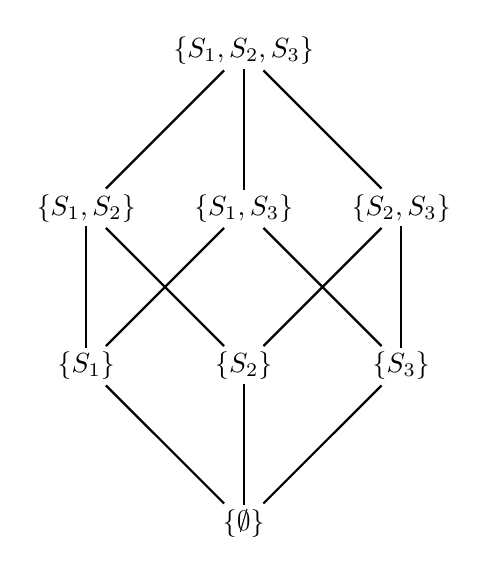
\begin{tikzpicture}
    % First, locate each of the nodes and name them
        \node (top) at (0,0) {$\{S_1, S_2, S_3\}$};
        \node (left) at (-2, -2) {$\{S_1, S_2\}$};
        \node (center) at (0, -2) {$\{S_1, S_3\}$};
        \node (right) at (2, -2) {$\{S_2, S_3\}$};
        \node (one) at (-2, -4) {$\{S_1\}$};
        \node (two) at (0, -4) {$\{S_2\}$};
        \node (three) at (2, -4) {$\{S_3\}$};
        \node (empty) at (0, -6) {$\{\emptyset \}$};

    % Now draw the lines:
        \draw [thick, shorten <=-2pt, shorten >=-2pt] (top) -- (left);
        \draw [thick, shorten <=-2pt, shorten >=-2pt] (top) -- (center);
        \draw [thick, shorten <=-2pt, shorten >=-2pt] (top) -- (right);
        \draw [thick, shorten <=-2pt, shorten >=-2pt] (left) -- (one);
        \draw [thick, shorten <=-2pt, shorten >=-2pt] (left) -- (two);
        \draw [thick, shorten <=-2pt, shorten >=-2pt] (center) -- (one);
        \draw [thick, shorten <=-2pt, shorten >=-2pt] (center) -- (three);
        \draw [thick, shorten <=-2pt, shorten >=-2pt] (right) -- (two);
        \draw [thick, shorten <=-2pt, shorten >=-2pt] (right) -- (three);
        \draw [thick, shorten <=-2pt, shorten >=-2pt] (one) -- (empty);
        \draw [thick, shorten <=-2pt, shorten >=-2pt] (two) -- (empty);
        \draw [thick, shorten <=-2pt, shorten >=-2pt] (three) -- (empty);
    \end{tikzpicture}   
    \caption{A Hesse Diagram for a world with 3 possible states}
    \label{fig:hesse}
\end{figure}
